\SourcePage{92}{95}
\section{The Linear Oscillator}

Consider a particle executing small one-dimensional oscillations (the
so-called \emph{linear oscillator}). Its potential energy is
$m\omega^2x^2/2$, where in classical mechanics $\omega$ is the natural
frequency of the oscillations. The oscillator Hamiltonian is consequently
\begin{equation}
  \hat H=\frac{\hat p^2}{2m}+\frac{m\omega^2x^2}{2}.
  \tag{23.1}
\end{equation}
Since the potential energy tends to infinity at $x=\pm\infty$, the particle
can execute only finite motion. Accordingly, the entire energy spectrum of
the oscillator is discrete.

Let us determine the oscillator's energy levels by the matrix
method\footnote{This was done by Heisenberg (1925), before Schrödinger's
discovery of the wave equation.}. We begin with the equations of motion in the
form (19.3), which in this case give
\begin{equation}
  \hat{\ddot x}+\omega^2x=0.
  \tag{23.2}
\end{equation}
In matrix form this equation is
\[
  (\ddot x)_{mn}+\omega^2x_{mn}=0.
\]
\SourcePage{93}{96}
For the matrix elements of the acceleration, (11.8) gives
$(\ddot x)_{mn}=i\omega_{mn}(\dot x)_{mn}=-\omega_{mn}^2x_{mn}$. Hence
\[
  (\omega_{mn}^2-\omega^2)x_{mn}=0.
\]
Thus all the matrix elements $x_{mn}$ vanish except those for which
$\omega_{mn}=\pm\omega$. Number all stationary states so that the frequencies
$\pm\omega$ correspond to the transitions $n\to n\mp1$, that is,
$\omega_{n,n\mp1}=\pm\omega$. The only nonzero matrix elements are then
$x_{n,n\mp1}$.

We shall suppose that the wave functions $\psi_n$ have been chosen real. Since
$x$ is a real quantity, every matrix element $x_{mn}$ is then real as well.
The Hermiticity condition (11.10) now makes the matrix $x_{mn}$ symmetric:
\[
  x_{mn}=x_{nm}.
\]

To calculate the nonzero coordinate matrix elements, use the commutation rule
\[
  \hat{\dot x}\,\hat x-\hat x\,\hat{\dot x}
  =-i\frac{\hbar}{m},
\]
written in matrix form as
\[
  (\dot x x)_{mn}-(x\dot x)_{mn}=-\frac{i\hbar}{m}\delta_{mn}.
\]
Using the matrix-multiplication rule (11.12), for $m=n$ this gives
\[
  i\sum_l(\omega_{nl}x_{nl}x_{ln}-x_{nl}\omega_{ln}x_{ln})
  =2i\sum_l\omega_{nl}x_{nl}^2=-\frac{i\hbar}{m}.
\]
Only the terms with $l=n\pm1$ are nonzero in this sum, and therefore
\begin{equation}
  (x_{n+1,n})^2-(x_{n,n-1})^2=\frac{\hbar}{2m\omega}.
  \tag{23.3}
\end{equation}
This equality shows that the quantities $(x_{n+1,n})^2$ form an arithmetic
progression, unbounded above but necessarily bounded below, since it can
contain only positive terms. Thus far we have established only the relative
ordering of the state labels $n$, not their absolute values; we may therefore
choose arbitrarily the value of $n$ assigned to the oscillator's first---the
normal---state. Set it equal to zero. Correspondingly, $x_{0,-1}$ must be
regarded as identically zero,
\SourcePage{94}{97}
and successive application of (23.3) for $n=0,1,\ldots$ gives
\[
  (x_{n,n-1})^2=\frac{n\hbar}{2m\omega}.
\]
The final expression for the nonzero coordinate matrix elements is
therefore\footnote{We choose the undetermined phases $\alpha_n$ (see the note
on p.~52) so that every matrix element in (23.4) has a plus sign before the
root. A phase convention of this kind can always be arranged when a matrix
has nonzero entries solely for transitions connecting states whose labels are
adjacent.}
\begin{equation}
  x_{n,n-1}=x_{n-1,n}=\sqrt{\frac{n\hbar}{2m\omega}}.
  \tag{23.4}
\end{equation}

The matrix of $\hat H$ is diagonal, and its matrix elements $H_{nn}$ are the
required oscillator energy eigenvalues $E_n$. To calculate them, write
\begin{align*}
  H_{nn}=E_n
  &=\frac m2\bigl[(\dot x^2)_{nn}+\omega^2(x^2)_{nn}\bigr]\\
  &=\frac m2\left[\sum_l i\omega_{nl}x_{nl}i\omega_{ln}x_{ln}
    +\omega^2\sum_lx_{nl}x_{ln}\right]
  =\frac m2\sum_l(\omega^2+\omega_{nl}^2)x_{ln}^2.
\end{align*}
Only the terms $l=n\pm1$ are nonzero in the sum. Substitution of (23.4) gives
\begin{equation}
  E_n=(n+1/2)\hbar\omega,\qquad n=0,1,2,\ldots
  \tag{23.5}
\end{equation}
Thus the oscillator energy levels are separated by equal intervals
$\hbar\omega$. The energy of the normal state ($n=0$) is $\hbar\omega/2$;
we emphasize that it is nonzero.

The result (23.5) may also be obtained by solving the Schrödinger equation.
For the oscillator this equation is
\begin{equation}
  \frac{d^2\psi}{dx^2}+\frac{2m}{\hbar^2}
  \left(E-\frac{m\omega^2x^2}{2}\right)\psi=0.
  \tag{23.6}
\end{equation}
It is convenient here to replace $x$ by a dimensionless variable $\xi$,
defined by
\begin{equation}
  \xi=\sqrt{\frac{m\omega}{\hbar}}x.
  \tag{23.7}
\end{equation}
\SourcePage{95}{98}
We then obtain
\begin{equation}
  \psi''+\left(\frac{2E}{\hbar\omega}-\xi^2\right)\psi=0.
  \tag{23.8}
\end{equation}
(A prime here denotes differentiation with respect to $\xi$.)

For large $\xi$, the term $2E/\hbar\omega$ may be omitted in comparison with
$\xi^2$; the equation $\psi''=\xi^2\psi$ has the asymptotic integrals
$\psi=e^{\pm\xi^2/2}$. (Indeed, differentiation of this function gives
$\psi''=\xi^2\psi$ when lower-order terms in $\xi$ are neglected.) Since the
wave function $\psi$ must remain finite at $\xi=\pm\infty$, the minus sign
must be chosen in the exponent. It is therefore natural to make the
substitution
\begin{equation}
  \psi=e^{-\xi^2/2}\chi(\xi)
  \tag{23.9}
\end{equation}
in (23.8). For $\chi(\xi)$ we obtain the equation (introducing the notation
$2E/\hbar\omega-1=2n$; since we know in advance that $E>0$, we have
$n>-1/2$)
\begin{equation}
  \chi''-2\xi\chi'+2n\chi=0,
  \tag{23.10}
\end{equation}
where $\chi$ must be finite for every finite $\xi$ and, at
$\xi=\pm\infty$, may become infinite no faster than a finite power of $\xi$
(so that $\psi$ tends to zero).

Such solutions of (23.10) exist only for integer positive values of $n$,
including zero (see \S~a of the mathematical supplements); this gives the
energy eigenvalues (23.5), already known to us. For the different integral
values of $n$, the corresponding solutions of (23.10) are
\[
  \chi=\operatorname{const}\cdot H_n(\xi),
\]
where $H_n(\xi)$ are the so-called Hermite polynomials, polynomials of degree
$n$ in $\xi$ defined by
\begin{equation}
  H_n(\xi)=(-1)^ne^{\xi^2}\frac{d^ne^{-\xi^2}}{d\xi^n}.
  \tag{23.11}
\end{equation}
Choosing the constant so that $\psi_n$ obeys the normalization condition
\[
  \int_{-\infty}^{+\infty}\psi_n^2(x)\,dx=1,
\]
we obtain (see (a.7))
\begin{equation}
  \psi_n(x)=\left(\frac{m\omega}{\pi\hbar}\right)^{1/4}
  \frac{1}{\sqrt{2^nn!}}
  \exp\left(-\frac{m\omega}{2\hbar}x^2\right)
  H_n\left(x\sqrt{\frac{m\omega}{\hbar}}\right).
  \tag{23.12}
\end{equation}
\SourcePage{96}{99}
Thus, the normal-state wave function is
\begin{equation}
  \psi_0(x)=\left(\frac{m\omega}{\pi\hbar}\right)^{1/4}
  \exp\left(-\frac{m\omega}{2\hbar}x^2\right).
  \tag{23.13}
\end{equation}
As expected, it has no zeros at finite $x$.

Evaluation of the integrals
$\int_{-\infty}^{+\infty}\psi_n\psi_m\xi\,d\xi$ determines the coordinate
matrix elements; the calculation naturally gives the same values (23.4).

We conclude by demonstrating how the wave functions $\psi_n$ can be computed
via the matrix method. In the matrices of the operators
$\hat{\dot x}\pm i\omega\hat x$, the only nonzero elements are
\begin{equation}
  (\dot x-i\omega x)_{n-1,n}=-(\dot x+i\omega x)_{n,n-1}
  =-i\sqrt{\frac{2\omega\hbar n}{m}}.
  \tag{23.14}
\end{equation}
Using the general formula (11.11) and recalling that $\psi_{-1}\equiv0$, we
obtain
\[
  (\hat{\dot x}-i\omega x)\psi_0=0.
\]
Substitution of $\hat{\dot x}=-i(\hbar/m)d/dx$ then gives
\[
  \frac{d\psi_0}{dx}=-\frac{m\omega}{\hbar}x\psi_0,
\]
whose normalized solution is (23.13). Further, since
\[
  (\hat{\dot x}+i\omega\hat x)\psi_{n-1}
  =(\dot x+i\omega x)_{n,n-1}\psi_n
  =i\sqrt{\frac{2\omega\hbar n}{m}}\psi_n,
\]
we obtain the recurrence formula
\begin{align*}
  \psi_n&=\sqrt{\frac{m}{2\omega\hbar n}}
  \left(-\frac{\hbar}{m}\frac d{dx}+\omega x\right)\psi_{n-1}
  =\frac1{\sqrt{2n}}\left(-\frac d{d\xi}+\xi\right)\psi_{n-1}\\
  &=-\frac1{\sqrt{2n}}\exp\frac{\xi^2}{2}\frac d{d\xi}
  \left(\exp\left(-\frac{\xi^2}{2}\right)\psi_{n-1}\right),
\end{align*}
whose $n$-fold application to (23.13) gives (23.12) for the normalized
functions $\psi_n$.

\ProblemHeading
\noindent\textbf{1.} Determine the probability distribution of the possible
momentum values for the oscillator.

\SolutionHeading
Rather than expanding a stationary-state wave function in momentum
eigenfunctions, for the oscillator it is simpler to begin directly with the
Schrödinger equation in the momentum representation. Substituting the
coordinate operator (15.12),
\SourcePage{97}{100}
$\hat x=i\hbar d/dp$, into (23.1), we obtain the Hamiltonian in the momentum
representation
\[
  \hat H=\frac{p^2}{2m}-\frac{m\omega^2\hbar^2}{2}\frac{d^2}{dp^2}.
\]
The corresponding Schrödinger equation $\hat Ha(p)=Ea(p)$ for the
momentum-representation wave function $a(p)$ is
\[
  \frac{d^2a(p)}{dp^2}+\frac{2}{m\omega^2\hbar^2}
  \left(E-\frac{p^2}{2m}\right)a(p)=0.
\]
This equation has exactly the same form as (23.6), so its solutions can be
written down directly by analogy with (23.12). The required probability
distribution is therefore
\[
  |a_n(p)|^2\frac{dp}{2\pi\hbar}
  =\frac{1}{2^nn!\sqrt{\pi m\omega\hbar}}
  \exp\left(-\frac{p^2}{m\omega\hbar}\right)
  H_n^2\left(\frac{p}{\sqrt{m\omega\hbar}}\right)dp.
\]

\ProblemHeading
\noindent\textbf{2.} Use the uncertainty relation (16.7) to determine a lower
bound on the possible energy values of the oscillator.

\SolutionHeading
Noting that $\overline{x^2}=\bar x^2+(\delta x)^2$ and
$\overline{p^2}=\bar p^2+(\delta p)^2$, and using (16.7), for the oscillator's
mean energy we have
\[
  \bar E=\frac{m\omega^2}{2}\overline{x^2}+\frac{\overline{p^2}}{2m}
  \geq\frac{m\omega^2}{2}(\delta x)^2+\frac1{2m}(\delta p)^2
  \geq\frac{m\omega^2\hbar^2}{8(\delta p)^2}+\frac{(\delta p)^2}{2m}.
\]
Finding the minimum of this expression as a function of $\delta p$, we obtain
the lower bound for the mean values, and hence for all possible energy values:
$E\geq\hbar\omega/2$.

\ProblemHeading
\noindent\textbf{3.} Find the wave functions of linear-oscillator states that
minimize the uncertainty relation, that is, states in which the
root-mean-square fluctuations of coordinate and momentum in the wave packet
are related by $\delta p\,\delta x=\hbar/2$ (E.~Schrödinger,
1926)\footnote{These states are called \emph{coherent}.}.

\SolutionHeading
The required wave functions must have the form
\begin{equation}
  \Psi(x,t)=\frac{1}{(2\pi)^{1/4}(\delta x)^{1/2}}
  \exp\left\{\frac{i\bar p x}{\hbar}
  -\frac{(x-\bar x)^2}{4(\delta x)^2}-i\varphi(t)\right\}.
  \tag{1}
\end{equation}
At every instant their coordinate dependence corresponds to (16.8), where
$\bar x=\bar x(t)$ and $\bar p=\bar p(t)=m\dot{\bar x}(t)$ are the mean
coordinate and momentum. By (19.3), for the linear oscillator
($U=m\omega^2x^2/2$) we have $\dot p=-m\omega^2x$, and hence for the mean
values $\dot{\bar p}=-m\omega^2\bar x$, or
\begin{equation}
  \ddot{\bar x}+\omega^2\bar x=0,
  \tag{2}
\end{equation}
that is, $\bar x(t)$ satisfies the classical equation of motion. The constant
factor in (1) is fixed by the normalization condition
$\int_{-\infty}^{\infty}|\Psi|^2dx=1$; besides this factor, $\Psi$ may contain
a phase factor with a time-dependent phase $\varphi(t)$. To find the unknown
$\delta x$ and the function $\varphi(t)$, we substitute (1) into
the wave equation
\[
  -\frac{\hbar^2}{2m}\frac{\partial^2\Psi}{\partial x^2}
  +\frac{m\omega^2x^2}{2}\Psi=i\hbar\frac{\partial\Psi}{\partial t}.
\]
\SourcePage{98}{101}
Taking account of (2), the substitution gives
\[
  \left(\frac{x^2}{2}-x\bar x\right)
  \left(\frac{m^2\omega^2}{\hbar^2}-\frac1{4(\delta x)^4}\right)
  +\left[\frac{m^2\dot{\bar x}^{2}}{2\hbar^2}
  -\frac{\bar x^2}{8(\delta x)^4}+\frac1{4(\delta x)^2}
  -\frac m\hbar\dot\varphi(t)\right]=0.
\]
It follows that $(\delta x)^2=\hbar/(2m\omega)$ and then
\[
  \dot\varphi=\frac m{2\hbar}(\dot{\bar x}^{2}-\omega^2\bar x^2)
  +\frac\omega2,
  \qquad
  \varphi=\frac1{2\hbar}\bar p\bar x+\frac\omega2t.
\]
Thus, finally,
\begin{equation}
  \Psi(x,t)=\left(\frac{m\omega}{\pi\hbar}\right)^{1/4}
  \exp\left\{\frac{i\bar p x}{\hbar}
  -\frac{m\omega(x-\bar x)^2}{2\hbar}\right\}
  \exp\left\{-\frac{i\omega t}{2}-\frac{i\bar p\bar x}{2\hbar}\right\}.
  \tag{3}
\end{equation}
For $\bar x=0$, $\bar p=0$, this function becomes
$\psi_0(x)e^{-i\omega t/2}$, the wave function of the oscillator ground state.

The oscillator's mean energy in a coherent state is
\begin{equation}
  \bar E=\frac{\overline{p^2}}{2m}+\frac{m\omega^2\overline{x^2}}{2}
  =\frac{\bar p^2}{2m}+\frac{m\omega^2\bar x^2}{2}+\frac{\hbar\omega}{2}
  =\hbar\omega\left(\bar n+\frac12\right);
  \tag{4}
\end{equation}
the quantity $\bar n$ introduced here is the mean ``number of quanta''
$\hbar\omega$ in the state. We see that a coherent state is specified
completely by giving a dependence $\bar x(t)$ that satisfies the classical
equation (2). Its general form can be written
\begin{equation}
  \frac{m\omega\bar x+i\bar p}{\sqrt{2m\hbar\omega}}
  =ae^{-i\omega t},\qquad |a|^2=\bar n.
  \tag{5}
\end{equation}
The function (3) may be expanded in the wave functions of the oscillator's
stationary states:
\[
  \Psi=\sum_{n=0}^{\infty}a_n\Psi_n,
  \qquad
  \Psi_n(x,t)=\psi_n(x)\exp\left\{-i\left(n+\frac12\right)\omega t\right\}.
\]
The coefficients of this expansion are\footnote{Compare the calculation in
Problem 1 of \secref{41}.}
\begin{equation}
  a_n=\int_{-\infty}^{\infty}\Psi_n^*\Psi\,dx.
  \tag{6}
\end{equation}
It follows that the probability for the oscillator to be in its $n$th state
is
\begin{equation}
  w_n=|a_n|^2=e^{-\bar n}\frac{\bar n^n}{n!},
  \tag{7}
\end{equation}
that is, it is given by the familiar Poisson distribution.

\ProblemHeading
\noindent\textbf{4.} Determine the energy levels of a particle moving in a
field with the potential energy shown in Fig.~3 (Ph.~Morse, 1929).

\SolutionHeading
The spectrum of positive energy eigenvalues is continuous (and the levels are
nondegenerate), while the spectrum of negative values is discrete.

The Schrödinger equation is
\[
  \frac{d^2\psi}{dx^2}+\frac{2m}{\hbar^2}
  (E-Ae^{-2\alpha x}+2Ae^{-\alpha x})\psi=0.
\]
\SourcePage{99}{102}
Introduce the new variable
\[
  \xi=\frac{2\sqrt{2mA}}{\alpha\hbar}e^{-\alpha x}
\]
(which ranges from zero to $+\infty$), and the notation (we consider the
discrete spectrum, so $E<0$)
\begin{equation}
  s=\frac{\sqrt{-2mE}}{\alpha\hbar},\qquad
  n=\frac{\sqrt{2mA}}{\alpha\hbar}-\left(s+\frac12\right).
  \tag{1}
\end{equation}
The Schrödinger equation then becomes
\[
  \psi''+\frac1\xi\psi'
  +\left(-\frac14+\frac{n+s+1/2}{\xi}-\frac{s^2}{\xi^2}\right)\psi=0.
\]
As $\xi\to\infty$, $\psi$ behaves asymptotically as $e^{\pm\xi/2}$, while as
$\xi\to0$ it is proportional to $\xi^{\pm s}$. Finiteness requires the
solution behaving as $e^{-\xi/2}$ at $\xi\to\infty$ and as $\xi^s$ at
$\xi\to0$.

\begin{center}
\begin{tikzpicture}[x=1.0cm,y=0.9cm]
  \draw[gray] (-2.2,0)--(2.5,0);
  \draw[gray] (0,-1.55)--(0,1.65);
  \draw[thick,domain=-0.85:2.25,samples=100,smooth]
    plot (\x,{exp(-2*\x)-2*exp(-\x)});
  \node[above right] at (0,1.45) {$U(x)$};
  \node[right] at (2.4,0) {$x$};
  \node[below left] at (0,-1) {$-A$};
\end{tikzpicture}

\small Fig.~3
\end{center}

Make the substitution
\[
  \psi=e^{-\xi/2}\xi^sw(\xi),
\]
which gives for $w$ the equation
\begin{equation}
  \xi w''+(2s+1-\xi)w'+nw=0,
  \tag{2}
\end{equation}
to be solved subject to the conditions that $w$ is finite at $\xi=0$, and
that as $\xi\to\infty$ it becomes infinite no faster than a finite power of
$\xi$. Equation (2) is the confluent hypergeometric equation (see \S~d of the
mathematical supplements),
\[
  w=F(-n,2s+1,\xi).
\]
The solution satisfying the required condition is obtained for a
nonnegative integer $n$ (and $F$ then reduces to a polynomial). From the
definitions (1), the energy levels are consequently
\[
  -E_n=A\left[1-\frac{\alpha\hbar}{\sqrt{2mA}}
  \left(n+\frac12\right)\right]^2,
\]
where $n$ takes integer positive values beginning at zero and ending at the
greatest value for which
\[
  \frac{\sqrt{2mA}}{\alpha\hbar}>n+\frac12
\]
(so that the parameter $s$ is positive, in agreement with its definition).
Thus the discrete spectrum contains a finite sequence of levels. If
\[
  \frac{\sqrt{2mA}}{\alpha\hbar}<\frac12,
\]
there is no discrete spectrum at all.

\ProblemHeading
\noindent\textbf{5.} The same problem for
$U=-U_0/\cosh^2\alpha x$ (Fig.~4).

\SolutionHeading
The positive-energy spectrum is continuous and the negative-energy spectrum
is discrete; we consider the latter. The Schrödinger equation is
\[
  \frac{d^2\psi}{dx^2}+\frac{2m}{\hbar^2}
  \left(E+\frac{U_0}{\cosh^2\alpha x}\right)\psi=0.
\]
\SourcePage{100}{103}
Make the change of variable $\xi=\tanh\alpha x$ and introduce the notation
\[
  \varepsilon=\frac{\sqrt{-2mE}}{\hbar\alpha},\qquad
  \frac{2mU_0}{\alpha^2\hbar^2}=s(s+1),\qquad
  s=\frac12\left(-1+\sqrt{1+\frac{8mU_0}{\alpha^2\hbar^2}}\right).
\]
We then obtain
\[
  \frac d{d\xi}\left[(1-\xi^2)\frac{d\psi}{d\xi}\right]
  +\left[s(s+1)-\frac{\varepsilon^2}{1-\xi^2}\right]\psi=0.
\]

\begin{center}
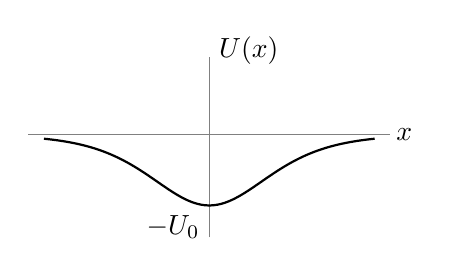
\begin{tikzpicture}[x=1.0cm,y=0.9cm]
  \draw[gray] (-2.3,0)--(2.3,0);
  \draw[gray] (0,-1.45)--(0,1.1);
  \draw[thick,domain=-2.1:2.1,samples=100,smooth]
    plot (\x,{-1/(cosh(\x)*cosh(\x))});
  \node[above right] at (0,0.85) {$U(x)$};
  \node[right] at (2.25,0) {$x$};
  \node[below left] at (0,-1) {$-U_0$};
\end{tikzpicture}

\small Fig.~4
\end{center}

This is the equation of the generalized Legendre functions. Reduce it to
hypergeometric form by the substitution
\[
  \psi=(1-\xi^2)^{\varepsilon/2}w(\xi)
\]
and the temporary change of variable $\tfrac12(1-\xi)=u$:
\[
  u(1-u)w''+(\varepsilon+1)(1-2u)w'
  -(\varepsilon-s)(\varepsilon+s+1)w=0.
\]
The solution finite at $\xi=1$ (that is, at $x=\infty$) is
\[
  \psi=(1-\xi^2)^{\varepsilon/2}
  F[\varepsilon-s,\varepsilon+s+1,\varepsilon+1,(1-\xi)/2].
\]
For $\psi$ to remain finite also at $\xi=-1$ (that is, at $x=-\infty$), we
must have $\varepsilon-s=-n$, where $n=0,1,2,\ldots$ (then $F$ is a
polynomial of degree $n$, finite at $\xi=-1$).

Thus the energy levels are fixed by $s-\varepsilon=n$, which gives
\[
  E_n=-\frac{\hbar^2\alpha^2}{8m}
  \left[-(1+2n)+\sqrt{1+\frac{8mU_0}{\alpha^2\hbar^2}}\right]^2.
\]
There is a finite number of levels, determined by the condition
$\varepsilon>0$, that is, $n<s$.
